\begin{frame}{Input: Lattice Graph}
  
    \begin{definition}
      A \textbf{lattice graph} is a strongly connected directed
      multi-graph in which each edge $e$ is labeled with a rigid body
      transformation $T(e)$ and each $\edge{v}{T(e)}{w}$ has an
      inverse edge $\edge{w}{T(e)^{-1}}{v}$.  
    \end{definition}
  
  \only<1>{\begin{columns}[T] % align columns
  \begin{column}{.45\textwidth}
    \begin{figure}
  \centering
  \begin{tikzpicture}[->,>=stealth',shorten >=5pt,auto,node distance=1cm]
    \tikzstyle{every state}=[fill=blue,draw=none, text=white]
    \node[state, scale=0.6] (A)         {$0$};
    \path (A) edge [loop above] node {\footnotesize{Tr(0, 40)}} (A)
    edge [loop left]  node {\footnotesize{Tr(-40,0)}} (A)
    edge [loop below] node {\footnotesize{Tr(0, -40)}} (A)
    edge [loop right] node {\footnotesize{Tr(40, 0)}} (A);
  \end{tikzpicture}
\end{figure}
  \end{column}%
  \begin{column}{.45\textwidth}
    \begin{figure}
      \centering
      \includegraphics[width=0.5\columnwidth]{figs/squarelattice}
    \end{figure}
  \end{column}%
\end{columns}}
  \only<2>{\begin{columns}[T] % align columns
  \begin{column}{.45\textwidth}
    \begin{figure}
    \centering
    \begin{tikzpicture}[scale=0.75, distance=1cm]
          %->,>=stealth',shorten >=5pt,auto,node          ]
          \tikzstyle{every state}=[fill=myred, draw=none, text=white]
          \node[state, scale=0.5] (A) at (0,0)    {$0$};
          \node[state, scale=0.5, fill=mycyan] (B) at (3,0)  {$1$};
          \path (A) edge [bend left=10] node {\scriptsize{Tr(0, 40)}} (B)
                (A) edge [bend left=45] node {\scriptsize{Tr(-35,-20)}} (B)
                (A) edge [bend left=90] node {\scriptsize{Tr(35,-20)}} (B)
                (B) edge [bend left=10] node {\scriptsize{Tr(-40,0)}} (A)
                (B) edge [bend left=45] node {\scriptsize{Tr(35,20)}} (A)
                (B) edge [bend left=90] node {\scriptsize{Tr(-35,20)}} (A);
    \end{tikzpicture}
\end{figure}
  \end{column}%
  \begin{column}{.45\textwidth}
    \begin{figure}
      \centering
      \includegraphics[width=0.5\columnwidth]{figs/hexagonlattice}
    \end{figure}
  \end{column}%
\end{columns}}
  \only<3>{\begin{columns}[T] % align columns
  \begin{column}{.45\textwidth}
    \begin{figure}
  \centering
  \begin{tikzpicture}[->,>=stealth',shorten >=5pt, node distance=5cm]
    \tikzstyle{every state}=[fill=myred, text=white, draw=none]
    %                  D
    %      C      A 
    % 
    %             B
    \node[state, scale=0.5] (A) at (0,0)    {$0$};
    \node[state, scale=0.5, fill=cyan] (B) at (0,-1)  {$1$};
    \node[state, scale=0.5, fill=blue] (C) at (-1,0)  {$2$};
    \node[state, scale=0.5, fill=orange] (D) at (1,1) {$3$};
    \path (A) edge (B) % node {\scriptsize{Tr(0, -40)}} (B)
    (A) edge (C) % node {\scriptsize{Tr(-40, 0)}} (C)
    (A) edge (D); % node {\scriptsize{Tr(28,28)}}  (D);
    \path (B) edge [bend left=10] (A)
    (B) edge (D) % node {\scriptsize{Tr(-40,0)}}  (D); 
    (B) edge (C); % node {\scriptsize{Tr(-28,28)}} (C);
    \path (C) edge [bend right=30] (B)
    (C) edge [bend left=10] (A)
    (C) edge [bend left=30] (D);
    \path (D) edge [bend left=30] (B)
    (D) edge [bend right=10] (A)
    (D) edge (C);
  \end{tikzpicture}
\end{figure}
  \end{column}%
  \begin{column}{.45\textwidth}
    \begin{figure}
      \centering
      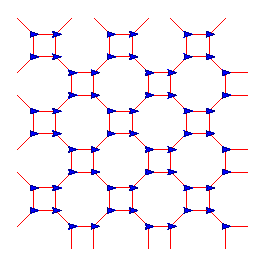
\includegraphics[width=0.5\columnwidth]{figs/octagonsquare}
    \end{figure}
  \end{column}%
\end{columns}}
\end{frame}